%set the master document for easy compilation
%!TEX root = ../D3_5_3.tex

\section{F2.8: Provide\_Position\_Report}\label{s:F2.8}

\subsection{Component Requirements}

\begin{longtable}{p{.25\textwidth}p{.7\textwidth}}
\toprule
Component name			& Provide\_Position\_Report \\
\midrule
Link to SCADE model		& {\footnotesize \url{https://github.com/openETCS/modeling/blob/master/model/Scade/System/ObuFunctions/ManageLocationRelatedInformation/TrainPosition/ProvidePositionReport/ProvidePositionReport_Pkg.xscade}}\\
\midrule
SCADE designer			& Christian Stahl, TWT GmbH \\
\midrule
Description				& The component builds a position report for the RBC, i.e., message 132, and provides it as an output.  There are two triggers for sending message 132:  
\begin{enumerate}
\item at least one of the triggers of the position report parameters (packet 58) holds or 
\item one of the events enabling the sending of the report occurs.
\end{enumerate} 
As the core position report (i.e., packet 0 or 1) is included in other packets, the
component also provides this core position report at every clock cycle. At most one of the two packets is valid.\\
\midrule
Input documents	& 
Subset-026, Chapter 3.6.5 \\
\midrule
Safety integrity level		& 4 \\
\midrule
Time constraints		& n/a
\\
\midrule
API requirements 		& n/a \\
\bottomrule
\end{longtable}


\subsection{Interface}

An overview of the interface of component Provide\_Position\_Report is shown in Figure~\ref{f:provide_position_report_interface}. The inputs and outputs are described in detail in Section~\ref{s:provide_position_report_inputs} respectively \ref{s:provide_position_report_outputs}. Subcomponents are described in Section~\ref{s:provide_position_report_subcomponents}.

\begin{figure}
\center
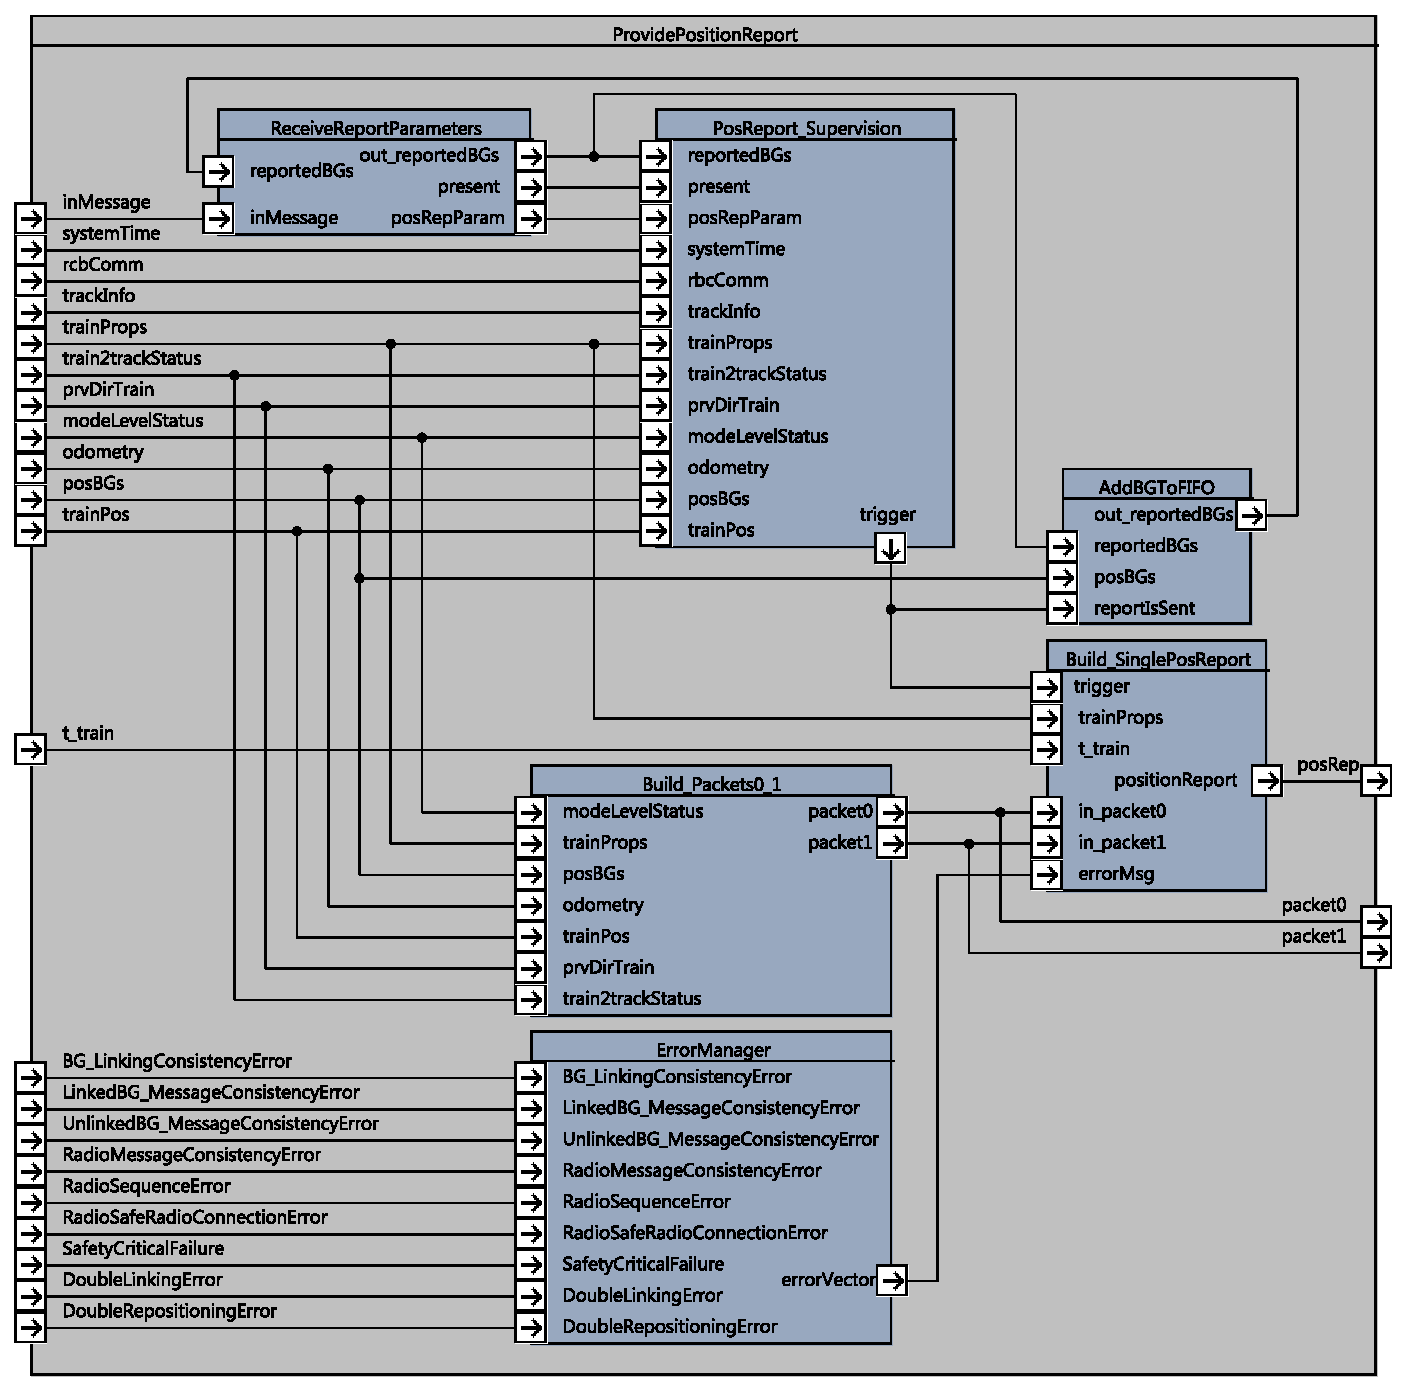
\includegraphics[width=\textwidth]{F2_8_ProvidePositionReport.pdf}
\caption{Provide\_Position\_Report component SysML diagram}\label{f:provide_position_report_interface}
\end{figure}


\subsubsection{Inputs}\label{s:provide_position_report_inputs}

\paragraph{inMessage}

\begin{longtable}{p{.25\textwidth}p{.7\textwidth}}
\toprule
Input name				& inMessage \\
\midrule
Description				& Input message from the bus (to extract Packet 58, the position report parameters). \\
\midrule
Source					& F2.1 Manage\_TrackSideInformation\_Integration\\ 
\midrule
Type					& Common\_Types\_Pkg::ReceivedMessage\_T \\
\midrule
Valid range of values	& as defined in SCADE \\
\midrule
Behaviour when value is at boundary	& n/a \\
\midrule
Behaviour for values out of valid range	& n/a \\
\midrule
Behaviour when value is erroneous, absent or unwanted (i.e. spurious) & If valid is false, then input is ignored. \\
\bottomrule
\end{longtable}


\paragraph{systemTime}

\begin{longtable}{p{.25\textwidth}p{.7\textwidth}}
\toprule
Input name				& systemTime \\
\midrule
Description				& The system time. \\
\midrule
Source					& F2 input API\_SystemTime \\ 
\midrule
Type					& SystemTime\_T, i.e., Obu\_BasicTypes\_Pkg::T\_internal\_Type \\
\midrule
Valid range of values	& [0; maximum positive int value of target platform] \\
\midrule
Behaviour when value is at boundary	& assumed to be valid \\
\midrule
Behaviour for values out of valid range	& assumed to be valid \\
\midrule
Behaviour when value is erroneous, absent or unwanted (i.e. spurious) & assumed to be valid \\
\bottomrule
\end{longtable}

\paragraph{rbcComm}

\begin{longtable}{p{.25\textwidth}p{.7\textwidth}}
\toprule
Input name				& rbcComm \\
\midrule
Description				& Variables modeling stati regarding the RBC communication. \\
\midrule
Source					& F2.9 MoRC\_HO \\ 
\midrule
Type					& RBC\_Communication\_T \\
\midrule
Valid range of values	& as defined in SCADE \\
\midrule
Behaviour when value is at boundary	& n/a \\
\midrule
Behaviour for values out of valid range	& n/a \\
\midrule
Behaviour when value is erroneous, absent or unwanted (i.e. spurious) & n/a \\
\bottomrule
\end{longtable}

\paragraph{trackInfo}

\begin{longtable}{p{.25\textwidth}p{.7\textwidth}}
\toprule
Input name				& trackInfo \\
\midrule
Description				& Location based events. \\
\midrule
Source					& EVC; currently a constant \\ 
\midrule
Type					& LocationBasedEvents\_T \\
\midrule
Valid range of values	& as defined in SCADE \\
\midrule
Behaviour when value is at boundary	& n/a \\
\midrule
Behaviour for values out of valid range	& n/a \\
\midrule
Behaviour when value is erroneous, absent or unwanted (i.e. spurious) & n/a \\
\bottomrule
\end{longtable}

\paragraph{trainProps}

\begin{longtable}{p{.25\textwidth}p{.7\textwidth}}
\toprule
Input name				& trainProps \\
\midrule
Description				& The train properties. \\
\midrule
Source					& F2.10 manageDMI\_Input \\ 
\midrule
Type					& TrainPosition\_Types\_Pck::trainProperties\_T \\
\midrule
Valid range of values	& as defined in SCADE \\
\midrule
Behaviour when value is at boundary	& n/a \\
\midrule
Behaviour for values out of valid range	& n/a \\
\midrule
Behaviour when value is erroneous, absent or unwanted (i.e. spurious) & n/a \\
\bottomrule
\end{longtable}

\paragraph{train2trackStatus}

\begin{longtable}{p{.25\textwidth}p{.7\textwidth}}
\toprule
Input name				& train2trackStatus \\
\midrule
Description				& Train to track status information. \\
\midrule
Source					& F2.10 manageDMI\_Input \\ 
\midrule
Type					& BG\_Types\_Pkg::TrainToTrackStatus\_T \\
\midrule
Valid range of values	& as defined in SCADE \\
\midrule
Behaviour when value is at boundary	& n/a \\
\midrule
Behaviour for values out of valid range	& n/a \\
\midrule
Behaviour when value is erroneous, absent or unwanted (i.e. spurious) & n/a \\
\bottomrule
\end{longtable}

\paragraph{prvDirTrain}

\begin{longtable}{p{.25\textwidth}p{.7\textwidth}}
\toprule
Input name				& prvDirTrain \\
\midrule
Description				& Train direction of the last clock cycle. \\
\midrule
Source					& F2.6 calculateTrainPosition \\ 
\midrule
Type					& Q\_DIRTRAIN \\
\midrule
Valid range of values	& as defined in SCADE \\
\midrule
Behaviour when value is at boundary	& n/a \\
\midrule
Behaviour for values out of valid range	& n/a \\
\midrule
Behaviour when value is erroneous, absent or unwanted (i.e. spurious) & n/a \\
\bottomrule
\end{longtable}

\paragraph{modeLevelStatus}

\begin{longtable}{p{.25\textwidth}p{.7\textwidth}}
\toprule
Input name				& modeLevelStatus \\
\midrule
Description				& Information referring to mode and level status. \\
\midrule
Source					& F2.5 ManageLevelAndMode \\ 
\midrule
Type					& ModeLevel2PositionReport\_T \\
\midrule
Valid range of values	& as defined in SCADE \\
\midrule
Behaviour when value is at boundary	& n/a \\
\midrule
Behaviour for values out of valid range	& n/a \\
\midrule
Behaviour when value is erroneous, absent or unwanted (i.e. spurious) & n/a \\
\bottomrule
\end{longtable}

\paragraph{odometry}

\begin{longtable}{p{.25\textwidth}p{.7\textwidth}}
\toprule
Input name				& odometry \\
\midrule
Description				& Odometry information.\\
\midrule
Source					& F2 input API\_Odometry \\ 
\midrule
Type					& Obu\_BasicTypes\_Pkg::odometry\_T \\
\midrule
Valid range of values	& as defined in SCADE \\
\midrule
Behaviour when value is at boundary	& n/a \\
\midrule
Behaviour for values out of valid range	& n/a \\
\midrule
Behaviour when value is erroneous, absent or unwanted (i.e. spurious) & n/a \\
\bottomrule
\end{longtable}

\paragraph{posBGs}

\begin{longtable}{p{.25\textwidth}p{.7\textwidth}}
\toprule
Input name				& posBGs \\
\midrule
Description				& Positioned balise groups used for current train position. \\
\midrule
Source					& F2.6 calculateTrainPosition \\ 
\midrule
Type					& TrainPosition\_Types\_Pck::positionedBGs\_T \\
\midrule
Valid range of values	& as defined in SCADE \\
\midrule
Behaviour when value is at boundary	& n/a \\
\midrule
Behaviour for values out of valid range	& n/a \\
\midrule
Behaviour when value is erroneous, absent or unwanted (i.e. spurious) & n/a \\
\bottomrule
\end{longtable}

\paragraph{trainPos}

\begin{longtable}{p{.25\textwidth}p{.7\textwidth}}
\toprule
Input name				& trainPos \\
\midrule
Description				& Current train position. \\
\midrule
Source					& F2.6 calculateTrainPosition \\ 
\midrule
Type					& TrainPosition\_Types\_Pck::trainPosition\_T \\
\midrule
Valid range of values	& as defined in SCADE \\
\midrule
Behaviour when value is at boundary	& n/a \\
\midrule
Behaviour for values out of valid range	& n/a \\
\midrule
Behaviour when value is erroneous, absent or unwanted (i.e. spurious) & n/a \\
\bottomrule
\end{longtable}

\paragraph{t\_train}

\begin{longtable}{p{.25\textwidth}p{.7\textwidth}}
\toprule
Input name				& t\_train \\
\midrule
Description				& Current timestamp. \\
\midrule
Source					& F2 input API\_persistentData \\ 
\midrule
Type					& T\_TRAIN \\
\midrule
Valid range of values	& as defined in SCADE \\
\midrule
Behaviour when value is at boundary	& n/a \\
\midrule
Behaviour for values out of valid range	& n/a \\
\midrule
Behaviour when value is erroneous, absent or unwanted (i.e. spurious) & n/a \\
\bottomrule
\end{longtable}

\paragraph{BG\_LinkingConsistencyError}

\begin{longtable}{p{.25\textwidth}p{.7\textwidth}}
\toprule
Input name				& BG\_LinkingConsistencyError \\
\midrule
Description				& True if respective error has occurred; otherwise false. \\
\midrule
Source					& F2.6 calculateTrainPosition \\ 
\midrule
Type					& bool \\
\midrule
Valid range of values	& as defined in SCADE \\
\midrule
Behaviour when value is at boundary	& n/a \\
\midrule
Behaviour for values out of valid range	& n/a \\
\midrule
Behaviour when value is erroneous, absent or unwanted (i.e. spurious) & n/a \\
\bottomrule
\end{longtable}

\paragraph{LinkedBG\_MessageConsistencyError}

\begin{longtable}{p{.25\textwidth}p{.7\textwidth}}
\toprule
Input name				& LinkedBG\_MessageConsistencyError \\
\midrule
Description				& True if respective error has occurred; otherwise false. \\
\midrule
Source					& F2.1 Manage\_TrackSideInformation\_Integration \\ 
\midrule
Type					& bool \\
\midrule
Valid range of values	& as defined in SCADE \\
\midrule
Behaviour when value is at boundary	& n/a \\
\midrule
Behaviour for values out of valid range	& n/a \\
\midrule
Behaviour when value is erroneous, absent or unwanted (i.e. spurious) & n/a \\
\bottomrule
\end{longtable}

\paragraph{UnlinkedBG\_MessageConsistencyError}

\begin{longtable}{p{.25\textwidth}p{.7\textwidth}}
\toprule
Input name				& UnlinkedBG\_MessageConsistencyError \\
\midrule
Description				& True if respective error has occurred; otherwise false. \\
\midrule
Source					& F2.1 Manage\_TrackSideInformation\_Integration \\ 
\midrule
Type					& bool \\
\midrule
Valid range of values	& as defined in SCADE \\
\midrule
Behaviour when value is at boundary	& n/a \\
\midrule
Behaviour for values out of valid range	& n/a \\
\midrule
Behaviour when value is erroneous, absent or unwanted (i.e. spurious) & n/a \\
\bottomrule
\end{longtable}

\paragraph{RadioMessageConsistencyError}

\begin{longtable}{p{.25\textwidth}p{.7\textwidth}}
\toprule
Input name				& RadioMessageConsistencyError \\
\midrule
Description				& True if respective error has occurred; otherwise false. \\
\midrule
Source					& F2.1Manage\_TrackSideInformation\_Integration \\ 
\midrule
Type					& bool \\
\midrule
Valid range of values	& as defined in SCADE \\
\midrule
Behaviour when value is at boundary	& n/a \\
\midrule
Behaviour for values out of valid range	& n/a \\
\midrule
Behaviour when value is erroneous, absent or unwanted (i.e. spurious) & n/a \\
\bottomrule
\end{longtable}

\paragraph{RadioSequenceError}

\begin{longtable}{p{.25\textwidth}p{.7\textwidth}}
\toprule
Input name				& RadioSequenceError \\
\midrule
Description				& True if respective error has occurred; otherwise false. \\
\midrule
Source					& F2.1 Manage\_TrackSideInformation\_Integration \\ 
\midrule
Type					& bool \\
\midrule
Valid range of values	& as defined in SCADE \\
\midrule
Behaviour when value is at boundary	& n/a \\
\midrule
Behaviour for values out of valid range	& n/a \\
\midrule
Behaviour when value is erroneous, absent or unwanted (i.e. spurious) & n/a \\
\bottomrule
\end{longtable}

\paragraph{RadioSafeRadioConnectionError}

\begin{longtable}{p{.25\textwidth}p{.7\textwidth}}
\toprule
Input name				& RadioSafeRadioConnectionError \\
\midrule
Description				& True if respective error has occurred; otherwise false. \\
\midrule
Source					& none; currently a constant \\ 
\midrule
Type					& bool \\
\midrule
Valid range of values	& as defined in SCADE \\
\midrule
Behaviour when value is at boundary	& n/a \\
\midrule
Behaviour for values out of valid range	& n/a \\
\midrule
Behaviour when value is erroneous, absent or unwanted (i.e. spurious) & n/a \\
\bottomrule
\end{longtable}

\paragraph{SafetyCriticalFailure}

\begin{longtable}{p{.25\textwidth}p{.7\textwidth}}
\toprule
Input name				& SafetyCriticalFailure \\
\midrule
Description				& True if respective error has occurred; otherwise false. \\
\midrule
Source					& EVC; currently a constant \\ 
\midrule
Type					& bool \\
\midrule
Valid range of values	& as defined in SCADE \\
\midrule
Behaviour when value is at boundary	& n/a \\
\midrule
Behaviour for values out of valid range	& n/a \\
\midrule
Behaviour when value is erroneous, absent or unwanted (i.e. spurious) & n/a \\
\bottomrule
\end{longtable}

\paragraph{DoubleLinkingError}

\begin{longtable}{p{.25\textwidth}p{.7\textwidth}}
\toprule
Input name				& DoubleLinkingError \\
\midrule
Description				& True if respective error has occurred; otherwise false. \\
\midrule
Source					& F2.6 calculateTrainPosition \\ 
\midrule
Type					& bool \\
\midrule
Valid range of values	& as defined in SCADE \\
\midrule
Behaviour when value is at boundary	& n/a \\
\midrule
Behaviour for values out of valid range	& n/a \\
\midrule
Behaviour when value is erroneous, absent or unwanted (i.e. spurious) & n/a \\
\bottomrule
\end{longtable}

\paragraph{DoubleRepositioningError}

\begin{longtable}{p{.25\textwidth}p{.7\textwidth}}
\toprule
Input name				& DoubleRepositioningError \\
\midrule
Description				& True if respective error has occurred; otherwise false. \\
\midrule
Source					& F2.6 calculateTrainPosition \\ 
\midrule
Type					& bool \\
\midrule
Valid range of values	& as defined in SCADE \\
\midrule
Behaviour when value is at boundary	& n/a \\
\midrule
Behaviour for values out of valid range	& n/a \\
\midrule
Behaviour when value is erroneous, absent or unwanted (i.e. spurious) & n/a \\
\bottomrule
\end{longtable}


\subsubsection{Outputs}\label{s:provide_position_report_outputs}

\paragraph{packet0}

\begin{longtable}{p{.25\textwidth}p{.7\textwidth}}
\toprule
Output name				& packet0 \\
\midrule
Description				& Packet 0 -- position report based on a single balise -- is provided every clock cycle. \\
\midrule
Destination				& F2.4 TrackAtlas\\ 
\midrule
Type					& Packet\_TrainTypes\_Pkg::PT0\_PositionReport\_T \\
\midrule
Valid range of values	& as defined in SCADE \\
\midrule
Behaviour when value is at boundary	& n/a \\
\midrule
Behaviour for values out of valid range	& n/a \\
\midrule
Behaviour when value is erroneous, absent or unwanted (i.e. spurious) & n/a \\
\bottomrule
\end{longtable}


\paragraph{packet1}

\begin{longtable}{p{.25\textwidth}p{.7\textwidth}}
\toprule
Output name				& packet1 \\
\midrule
Description				& Packet 1 -- position report based on two balise groups -- is provided every clock cycle. \\
\midrule
Destination				& F2.4 TrackAtlas \\ 
\midrule
Type					& Packet\_TrainTypes\_Pkg::PT1\_PositionReport\_2BG\_T \\
\midrule
Valid range of values	& as defined in SCADE \\
\midrule
Behaviour when value is at boundary	& n/a \\
\midrule
Behaviour for values out of valid range	& n/a \\
\midrule
Behaviour when value is erroneous, absent or unwanted (i.e. spurious) & n/a \\
\bottomrule
\end{longtable}

\paragraph{posRep}

\begin{longtable}{p{.25\textwidth}p{.7\textwidth}}
\toprule
Output name				& posRep \\
\midrule
Description				& Position report to be send to the RBC, i.e. message 136. \\
\midrule
Destination				& F2 output API\_toEuroradio \\ 
\midrule
Type					& Radio\_Types\_Pkg::Radio\_TrainTrack\_Message\_T \\
\midrule
Valid range of values	& as defined in SCADE \\
\midrule
Behaviour when value is at boundary	& n/a \\
\midrule
Behaviour for values out of valid range	& n/a \\
\midrule
Behaviour when value is erroneous, absent or unwanted (i.e. spurious) & n/a \\
\bottomrule
\end{longtable}


\subsection{Subcomponents}\label{s:provide_position_report_subcomponents}


\subsubsection{ReceiveReportParameters}
%set the master document for easy compilation
%!TEX root = ../D3_5_3.tex

\paragraph{Component Requirements}

\begin{longtable}{p{.25\textwidth}p{.7\textwidth}}
\toprule
Component name			& ReceiveReportParameters \\
\midrule
Link to SCADE model		& {\footnotesize \url{http://???}} \\
\midrule
SCADE designer			& Christian Stahl, TWT \\
\midrule
Description				& The component reads the position report parameters (i.e., packet 58) from the message bus. When a report is received, the BG information provided is used to update the location of respective BG. This BG is being stored in the list of the last 8 BGs. \\
\midrule
Input documents	& 
Subset-026, Chapter ?.?\newline
Subset-026, Chapter ?.?\newline
Subset-026, Chapter ?.?.?\\
\midrule
Safety integrity level		& 4 \\
\midrule
Time constraints		& [If applicable description of time constraints, otherwise n/a] \\
\midrule
API requirements 		& [If applicable description of API requirements, otherwise n/a] \\
\bottomrule
\end{longtable}


\paragraph{Interface}

For an overview of the interface of this internal component we refer to the SCADE model (cf.~link above) respectively the SCADE generated documentation.

\subsubsection{PosReport\_Supervision}
%set the master document for easy compilation
%!TEX root = ../D3_5_3.tex

\paragraph{Component Requirements}

\begin{longtable}{p{.25\textwidth}p{.7\textwidth}}
\toprule
Component name			& PosReport\_Supervision \\
\midrule
Link to SCADE model		& {\footnotesize \url{http://???}} \\
\midrule
SCADE designer			& Christian Stahl, TWT \\
\midrule
Description				& The component supervises trigger (i.e., position report parameter) and events that trigger the sending of a position report. If the output is true, then a report has to be sent. \\
\midrule
Input documents	& 
Subset-026, Chapter ?.?\newline
Subset-026, Chapter ?.?\newline
Subset-026, Chapter ?.?.?\\
\midrule
Safety integrity level		& 4 \\
\midrule
Time constraints		& [If applicable description of time constraints, otherwise n/a] \\
\midrule
API requirements 		& [If applicable description of API requirements, otherwise n/a] \\
\bottomrule
\end{longtable}


\paragraph{Interface}

For an overview of the interface of this internal component we refer to the SCADE model (cf.~link above) respectively the SCADE generated documentation.

\subsubsection{ErrorManager}
%set the master document for easy compilation
%!TEX root = ../D3_5_3.tex

\paragraph{Component Requirements}

\begin{longtable}{p{.25\textwidth}p{.7\textwidth}}
\toprule
Component name			& ErrorManager \\
\midrule
Link to SCADE model		& {\footnotesize \url{http://???}} \\
\midrule
SCADE designer			& Christian Stahl, TWT \\
\midrule
Description				& The component takes all nine possible error messages as an input and aggregates them to a vector. \\
\midrule
Input documents	& 
Subset-026, Chapter ?.?\newline
Subset-026, Chapter ?.?\newline
Subset-026, Chapter ?.?.?\\
\midrule
Safety integrity level		& 4 \\
\midrule
Time constraints		& [If applicable description of time constraints, otherwise n/a] \\
\midrule
API requirements 		& [If applicable description of API requirements, otherwise n/a] \\
\bottomrule
\end{longtable}


\paragraph{Interface}

For an overview of the interface of this internal component we refer to the SCADE model (cf.~link above) respectively the SCADE generated documentation.

\subsubsection{Build\_Packets0\_1}
%set the master document for easy compilation
%!TEX root = ../D3_5_3.tex

\paragraph{Component Requirements}

\begin{longtable}{p{.25\textwidth}p{.7\textwidth}}
\toprule
Component name			& Build\_Packets0\_1 \\
\midrule
Link to SCADE model		& {\footnotesize \url{https://github.com/openETCS/modeling/blob/master/model/Scade/System/ObuFunctions/ManageLocationRelatedInformation/TrainPosition/ProvidePositionReport/ProvidePositionReport_Pkg.xscade}} \\
\midrule
SCADE designer			& Christian Stahl, TWT \\
\midrule
Description				& The component builds packets 0 and 1; at most one of them is valid. \\
\midrule
Input documents	& 
Subset-026, Chapter 3.6.5 \\
\midrule
Safety integrity level		& 4 \\
\midrule
Time constraints		& n/a \\
\midrule
API requirements 		& n/a \\
\bottomrule
\end{longtable}


\paragraph{Interface}

For an overview of the interface of this internal component we refer to the SCADE model (cf.~link above) respectively the SCADE generated documentation.

\subsubsection{Build\_PosReport}
%set the master document for easy compilation
%!TEX root = ../D3_5_3.tex

\paragraph{Component Requirements}

\begin{longtable}{p{.25\textwidth}p{.7\textwidth}}
\toprule
Component name			& Build\_PosReport \\
\midrule
Link to SCADE model		& {\footnotesize \url{https://github.com/openETCS/modeling/blob/master/model/Scade/System/ObuFunctions/ManageLocationRelatedInformation/TrainPosition/ProvidePositionReport/ProvidePositionReport_Pkg.xscade}} \\
\midrule
SCADE designer			& Christian Stahl, TWT \\
\midrule
Description				& This operator builds nine position report messages -- there can be up to nine errors, and for each error an individual report has to be sent.
The fold operator ensures that the first report is invalid if the first error is not present but there exists an error in the error field. In other words,
one valid report will be built. If the errorVector does not contain a single error, 
then at least one report needs to be built (if the operator is triggered). \\
\midrule
Input documents	& 
Subset-026, Chapter 3.6.5 \\
\midrule
Safety integrity level		& 4 \\
\midrule
Time constraints		& n/a
\\
\midrule
API requirements 		& n/a \\
\bottomrule
\end{longtable}


\paragraph{Interface}

For an overview of the interface of this internal component we refer to the SCADE model (cf.~link above) respectively the SCADE generated documentation.

\subsubsection{AddBGToFIFO}
%set the master document for easy compilation
%!TEX root = ../D3_5_3.tex

\paragraph{Component Requirements}

\begin{longtable}{p{.25\textwidth}p{.7\textwidth}}
\toprule
Component name			& AddBGToFIFO \\
\midrule
Link to SCADE model		& {\footnotesize \url{http://???}} \\
\midrule
SCADE designer			& Christian Stahl, TWT \\
\midrule
Description				&  The component adds the current reported BG to the list of BGs for which a report has been sent. Adding of this BG is performed according to the FIFO method. \\
\midrule
Input documents	& 
Subset-026, Chapter ?.?\newline
Subset-026, Chapter ?.?\newline
Subset-026, Chapter ?.?.?\\
\midrule
Safety integrity level		& 4 \\
\midrule
Time constraints		& [If applicable description of time constraints, otherwise n/a] \\
\midrule
API requirements 		& [If applicable description of API requirements, otherwise n/a] \\
\bottomrule
\end{longtable}


\paragraph{Interface}

For an overview of the interface of this internal component we refer to the SCADE model (cf.~link above) respectively the SCADE generated documentation.

